\lecdate{20.03.2017}
\slides[0.5]{STTI_intro_2017}{6}
% Passwort: Tallinn11
\section{Einführung}
\subsection*{Ziel der Vorlesung}
\slides{reliability/contents}{2}
\subsection{Zuverlässige / fehlertolerante Systeme}
\slides{reliability/contents}{4}
Einfachstes Mittel für besser Reliability: \emph{Redundanz}\\
Failur classes … meint Fehler-Klassen von kritischen Fehlern (Versagen)
\subsection{Modellierung fehlertoleranter Systeme}
\slides{reliability/contents}{5}

\section{Grundlegende Zuverlässigkeitsquantifizierung}
\slides{reliability/contents}{3}
Reliability … Zuverlässigkeit / Wahrscheinlichkeit, dass ein System über eine Zeit funktionsfähig ist\\
Availability … Verfügbarkeit (pro Zeit)\\
Mission time … Wie lange soll ein System ohne Reparatur „im Feld“ bleiben?

\subsection{Wie lang läuft ein System ohne Versagen?}
\slides{reliability/part1}{3}
\slides{reliability/part1}{4}
Also: Der Mittelwert gibt keine Garantie, dass das Gerät bis zu einer bestimmten Zeit läuft.

\subsection{Wie Wahrscheinlich ist die fehlerfreie Nutzung für einen bestimmten Zeitraum?}
\slides{reliability/part1}{5}
\slides{reliability/part1}{6}

\subsection{Versagenswahrscheinlichkeit und Zuverlässigkeit}
\slides{reliability/part1}{7}
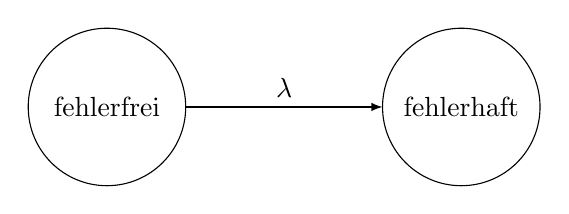
\begin{tikzpicture}
\draw  (-4.5,0) node{fehlerfrei} circle (1);
\draw  (0,0)  node{fehlerhaft} circle (1);
\draw[-latex] (-3.5,0) -- (-1,0) node[pos=.5, above]{$\lambda$};
\end{tikzpicture}\\
$R(t)=P(fehlerfrei)$\\
$R(t)=e^{-\lambda t}$\\
$R'(t)=-\lambda R(t)$

\subsection{Mittlere Zeit bis zum Versagen (MTTF)}
\slides{reliability/part1}{8}
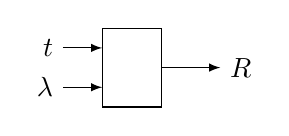
\begin{tikzpicture}[scale=.5]
\draw  (-1.5,2) rectangle (0,0);
\draw [-latex] (-2.5,1.5) node[left]{$t$} -- (-1.5,1.5);
\draw [latex-] (-1.5,0.5) -- (-2.5,0.5) node[left]{$\lambda$};
\draw [-latex] (0,1) -- (1.5,1) node[right]{$R$};
\end{tikzpicture}\\
$MTTF=P(L>t)=E(t)=\frac{1}{\lambda}$\\
Bspw.: $\lambda=5 \frac{1}{year} \to MTTF=\frac{1}{5}year$

\subsection{Verfügbarkeit}
\slides{reliability/part1}{9}
\slides{reliability/part1}{10}

\subsection{Beispiel Versagen und Verfügbarkeit}
\subsubsection{Einzelne Komponente ohne Reparatur}
\slides{reliability/part1}{11}
Die Einsatzdauer sollte immer deutlich kürzer sein, als die MTTF (da $R(MTTF)=0,37$ -- also die Fehlerrate zur mittleren Versagenszeit -- ein sehr schlechter Wert ist).
\subsubsection{Einzelne Komponente mit Reparatur}
\slides{reliability/part1}{12}

\subsection{Systemstruktur}
\slides{reliability/part1}{13}

